


\chapter{الدراسة المرجعية}
يبيّن هذا الفصل الدراسة المرجعية للمشروع.
يبدأ بتقديم مفاهيم تعلّم الآلة ومراحلها المختلفة والمعايير المعتمدة لتقييمها.
ويقدّم مفاهيم ومراحل معالجة اللغات الطبيعية.
وأخيراً يسرد بعض الأوراق الأبحاث العلمية المتعلقة بهذا المشروع، ويوضح المنهجيات المتبعة فيها.







\section{تعلم الآلة}
تعلم الآلة \textenglish{Machine Learning} هو فرع جزئي من الذكاء الصنعي \textenglish{Artificial Intelligence}.
يُقصد بتعلم الآلة مجموعة الأدوات والمفاهيم والمنهجيات المستخدمة لبرمجة الحواسيب
بطريقة تسمح لهذه الحواسيب بالتعلم من المعطيات.

ويمكن أيضاً تعريفه بشكل أكثر عمومية كالتالي:

\begin{english}
	``Machine Learning is the field of study that gives computers the ability to learn
	without being explicitly programmed.'' \\
	--Arthur Samuel, 1959
\end{english}

كما يعتبر التعريف التالي تقني وأكثر دقة:

\begin{english}
	``A computer program is said to learn from experience $E$ with respect to some task $T$
	and some performance measure $P$, if its performance on $T$, as measured by $P$, improves
	with experience $E$.'' \\
	--Tom Mitchell, 1997
\end{english}

على سبيل المثال، النظام الذي يقوم بفلترة الإيميلات إلى إيميلات مؤذية \textenglish{spam} وإيميلات غير مؤذية \textenglish{non-spam}، يستخدم منهجيات تعلم الآلة.
يقوم هذا النظام بتعلم طريقة التمييز بين هذين النوعين من الإيميلات باستخدام عدد كبير من الأمثلة والمعطيات المصنفة مسبقاً.
نسمي هذه المجموعة من الأمثلة بمعطيات التدريب \textenglish{Training Set}، وكل مثال منها نسميه مثال تدريبي \textenglish{Training Instance}.

في هذه الحالة، المهمة $T$ هي تصنيف الإيميلات الجديدة إلى إيميلات مؤذية وإيميلات غير مؤذية، الخبرة $E$ هي مجموعة معطيات التدريب،
ومؤشر قياس الأداء $P$ يمكن تعريفه بعدّة طرق؛ فمثلاً يمكننا استخدام نسبة نسبة عدد الإيميلات التي تم تصنيفها بشكل صحيح إلى عدد الإيميلات الكلي
(هذا المعيار يسمى الصِحَّة \textenglish{Accuracy} كم سنرى لاحقاً).

\subsection{تصنيفات تعلم الآلة}
\label{sec:ml:classification}
يمكن تصنيف أنظمة تعلم الآلة وفق عدّة معايير. التصنيف الأكثر شهرة يعتمد على آلية التدريب، وهو كالتالي:
\begin{itemize}
	\item
	التعلم تحت الإشراف \textenglish{Supervised Learning}:
	وهي حالة أن تكون الأمثلة التدريبية متوفرة مع الخرج \textenglish{label} المرتبط بها. وهذه حالة مثال تصنيف الإيميلات المطروح سابقاً.
	حيث أن معطيات التدريب هي مجموعة كبيرة من الإيميلات المصنفة مسبقاً من قبل البشر إلى إيميلات مؤذية وإيميلات غير مؤذية.
	\item
	التعلم بدون إشراف \textenglish{Unsupervised Learning}:
	وهي حالة أن تكون معطيات التدريب موجودة ولكنها غير مصنفة \textenglish{unlabeled} أو غير مرتبطة بخرج معيّن.
	على سبيل المثال، قد ترغب شركة في تصنيف زبائنها إلى عدّة مستويات، زبائن من الدرجة الأولى، زبائن من الدرجة الثانية، وهكذا.
	فيمكن استخدام تعلم الآلة لاكتشاف بعض الأنماط الموجودة في معطيات الزبائن واكتشاف هكذا تصنيف.
	وهذا ما يُعرف بالتجميع \textenglish{Clustering}.
	\item
	التعلم نصف المشرف عليه \textenglish{Semi-Supervised Learning}:
	وهي حالة وسيطة بين التصنيفين السابقين. تكون فيها بعض أمثلة التدريب مرتبطة بخرج معيّن (غالباً تشكل النسبة الصغيرة)،
	وتكون باقي الأمثلة غير مرتبطة بخرج. تنطبق هذه الحالة على مثال تصنيف الإيميلات في حال لم تكن جميع معطيات التدريب مصنفة بشكل مسبق.
	\item 
	التعلم بالتعزيز \textenglish{Reinforcement Learning}:
	وهي الحالة التي يتخاطب فيها النظام مع بيئة أخرى. تقدم له هذه البيئة نتائج \textenglish{feedback} بناءً على أفعاله.
	هذا الصنف ينطبق على الخوارزميات المستخدمة لتدريب الأنظمة التي تتعلم الألعاب.
	حيث يقوم النظام بمجموعة من الأفعال \textenglish{actions} ضمن بيئة اللعبة،
	وبناءً على النتائج (تحسّن نتيجته أو انخفاضها) يغيّر أفعاله اللاحقة.
\end{itemize}

وعلى وجه الخصوص يمكن تصنيف التعلم تحت الإشراف بحسب نوع الخرج المرتبط بمعطيات التدريب.
تصنّف بشكل أساسي عريض كالتالي:
\begin{itemize}
	\item 
	التصنيف \textenglish{Classification}:
	يكون الخرج المرتبط بكل مثال تدريبي هو صف \textenglish{class} محدد من مجموعة صفوف. عدد هذه الصفوف قد يكون $2$، $3$، إلخ.
	في مثال تصنيف الإيميلات السابق، عدد الصفوف هو $2$، حيث أن كل مثال تدريبي (إيميل معيّن من معطيات التدريب) هو إمّا مؤذي أو غير مؤذي.
	\item 
	الانحدار \textenglish{Regression}:
	يكون الخرج المرتبط بكل مثال تدريبي هو عدد حقيقي. مثل مسألة التنبؤ بسعر منزل بمعرفة معلومات عنه مثل مساحته، عدد الغرف، إلخ.
\end{itemize}






\subsection{المراحل اللازمة لتطبيق تعلم الآلة}
\label{sec:ml:steps}
إذا عدنا إلى مثال تصنيف الإيميلات، حيث قلنا أن معطيات التدريب هي مجموعة من الإيميلات المصنفة بشكل مسبق إلى إيميلات مؤذية وإيميلات غير مؤذية.
يمكن أن نسأل هنا: ما هو تحديداً الدخل؟ أي كيف سنعبّر عن الإيميل؟ بالطبع يمكن اعتبار الإيميل كنص؛ فهو مجموعة من الكلمات والرموز.
ولكن كما سنرى لاحقاً، من الصعب على معظم خوارزميات تعلم الآلة التعامل مع نص خام. ولذلك هناك مرحلة تسبق مرحلة تنفيذ خوارزميات تعلم الآلة
وهي مرحلة تحويل النص إلى ما يسمى بالميزات \textenglish{Features}.

فمثلاً يمكن أن نعبّر عن نص الإيميل بميزاته، مثل عدد الكلمات، عدد الجمل،
تواتر وجود كلمات مفتاحية محددة، إلخ. نلاحظ الآن في هذه الحالة أننا نتعامل مع الإيميل كشعاع من الميزات \textenglish{feature vector} وهذا أمر مناسب جداً
للعديد من خوارزميات تعلم الآلة. أيضاً إن الميزات التي ذكرناها هي ميزات عددية \textenglish{numerical features}، ولكن بشكل عام يمكن أن تكون الميزات
هي ميزات نصية \textenglish{string features} أو ميزات صنفية \textenglish{categorical features}، إلخ. ويمكن أيضاً تنميط الميزات بشكل مختلف أو أكثر دقة
مثل تصنيف الميزات العددية إلى ميزات مستمرة \textenglish{continuous features} وميزات متقطعة \textenglish{discrete features}. وتعود طريقة التنميط إلى
التطبيق أو خوارزميات تعلم الآلة المستخدمة. تسمى هذه المرحلة بمرحلة استخراج الميزات \textenglish{Feature Extraction}.

في التطبيقات الواقعية تسبق المرحلة السابقة مرحلتين أساسيتين. مرحلة تجميع المعطيات، ومرحلة تنظيفها. تتم عملية تجميع المعطيات بحسب التطبيق.
فمثلاً قد تكون المعطيات هي نتيجة استبيانات، أو إحصائيات، أو تم الحصول عليها من مواقع إلكترونية، إلخ.
مرحلة تنظيف المعطيات تهدف إلى التأكد سلامة المعطيات قبل استخدامها. وقد تتم هذه العملية بشكل يدوي أو بشكل مؤتمت وذلك بحسب مصدر المعطيات ونظافتها.




\subsection{خوارزميات تعلم الآلة}
كما رأينا في الفقرة~\ref{sec:ml:classification}، هناك العديد من أصناف المسائل الممكن حلها باستخدام تعلم الآلة.
تصنف خوارزميات تعلم الآلة تبعاً لصنف المسألة التي تقوم بحلها. فمثلاً يمكن استخدام الانحدار الخطي
\textenglish{Linear Regression}
لحل مسائل الانحدار~\cite{hands-on}.
أو استخدام خوارزمية \textenglish{K-Means Clustering}  لحل مسائل التجميع~\cite{hands-on}.
سنمهد في هذه الفقرة لأهم خوارزمية مستخدمة في هذا المشروع.
وهي الـ \textenglish{SVM}.


\subsubsection{خوارزمية الـ \LR{SVM}}
إن كلمة \textenglish{SVM} هي اختصار لـ \textenglish{Support Vector Machine}.
وهي خوارزمية تصنيف شهيرة وواسعة الاستخدام في تطبيقات تعلم الآلة.
تعتبر خوارزمية قوية حيث أنها تستند على أساس رياضي متين، ولها عدد من الخصائص المهمّة.
يمكن تقديم هذه الخوارزمية بعدّة طرق.
سنقدمها بطرح مسألة الأملثة التي تقوم بحلها.

بدايةً لنفرض أن مسألتنا هي مسألة تصنيف وعدد الصفوف هو $2$.
نرمز بـ
$(x^{(i)}, y^{(i)})_{1 \leq i \leq m}$
إلى معطيات التدريب.
حيث $m$ عدد معطيات التدريب.
ويكون المثال التدريبي رقم $i$، له الصف $ y^{(i)} $.
مع كون $ y^{(i)} = +1 $ في حال الصف الأول، و $ y^{(i)} = -1 $ في حال الصف الثاني.
وإن $ x^{(i)} $ هو شعاع عددي بـ $ n+1 $ بُعد أي
$ x^{(i)} \in \mathbb{R}^{n+1} $%
. وهو ما سميناه شعاع الميزات في الفقرة \ref{sec:ml:steps}.
أي هنا لدينا $n$ ميزة، حيث لتبسيط العلاقات الرياضية نضيف $ x^{(i)}_0 = 1 $.

النموذج المطروح في خوارزمية الـ \textenglish{SVM}، هو تعريف تابع 
$ f: \mathbb{R}^{n+1} \rightarrow \{-1, +1 \} $%
. حيث أننا نقول أنه لأجل عيّنة ما $ (x, y) $، فإنها تنتمي إلى الصف الأول في حال كان $ f(x) \geq 0 $،
وتنتمي إلى الصف الثاني في حال $ f(x) < 0 $.
سنأخذ مبدئياً للتبسيط التابع $f$ بالشكل
$ f(x) = \theta_0 x_0 + \theta_1 x_1 + \dots + \theta_n x_n $
حيث
$ \theta = (\theta_j)_{0 \leq j \leq n} $
هي البارامترات التي يمكن تغييرها.

مسألة الأمثلة التي نريد حلها هي:
\begin{align}
\label{eq:svm:primal}
&
\argmin_{\theta \in \mathbb{R}^{n+1} } \left(
\norm{\theta}^2 +
C \cdot \sum_{i = 1}^{m} \pospart{1 - y^{(i)} f(x^{(i)})}
\right)
\\
&
\mathrm{where}
f(x^{(i)}) = \sum_{j = 0}^{n} \theta_j x^{(i)}_j
\nonumber
\end{align}
حيث أن التابع
$\pospart{\cdot}$
هو تابع الجزء الموجب؛ أي
$ \pospart{z} = \max(z, 0) $%
. و
$ \norm{\cdot} $
هو النظيم الإقليدي؛ أي
$ \norm{\theta}^2 = \sum_{j=0}^{n} \theta_j^2 $%
. والباراميتر $C$ هو معامل وزن، يحدد مدى التفضيل والمساومة بين الحديّن الأول والثاني في المعادلة.
وهو باراميتر فوقي \eng{Hyperparameter} أي يجب تحديده قبل البدء بحل مسألة الأمثلة، وإن تغييره يغيير حل المسألة.

إن الحد الأول $ \norm{\theta}^2 $ في المعادلة \ref{eq:svm:primal} هو للتنظيم \textenglish{Regularization}.
هذا الحد يضبط قيم البارميتر $ \theta $ ويمنعها من أن تأخذ قيم كبيرة.
الحد الثاني يمثل مجموع قيمة الخطأ الحاصل في كل مثال تدريبي من معطيات التدريب.
حيث أن الخطأ الحاصل في عيّنة ما $ (x, y) $ هو
 $ \pospart{1 - y \cdot f(x)} $%
. يمكن تأمل صفات هذا الخطأ من خلال الشكل~\ref{fig:svm:error}.
حيث نلاحظ مثلاً في حالة $ y = 1 $ أن الخطأ يساوي الصفر عندما $ f(x) \geq 1 $ 
وأنه يتزايد بشكل خطي كلما أبتعدت قيمة $ f(x) $ عن $1$ بالاتجاه الخاطئ.
 \begin{figure}[htb] 
 	\centering
 	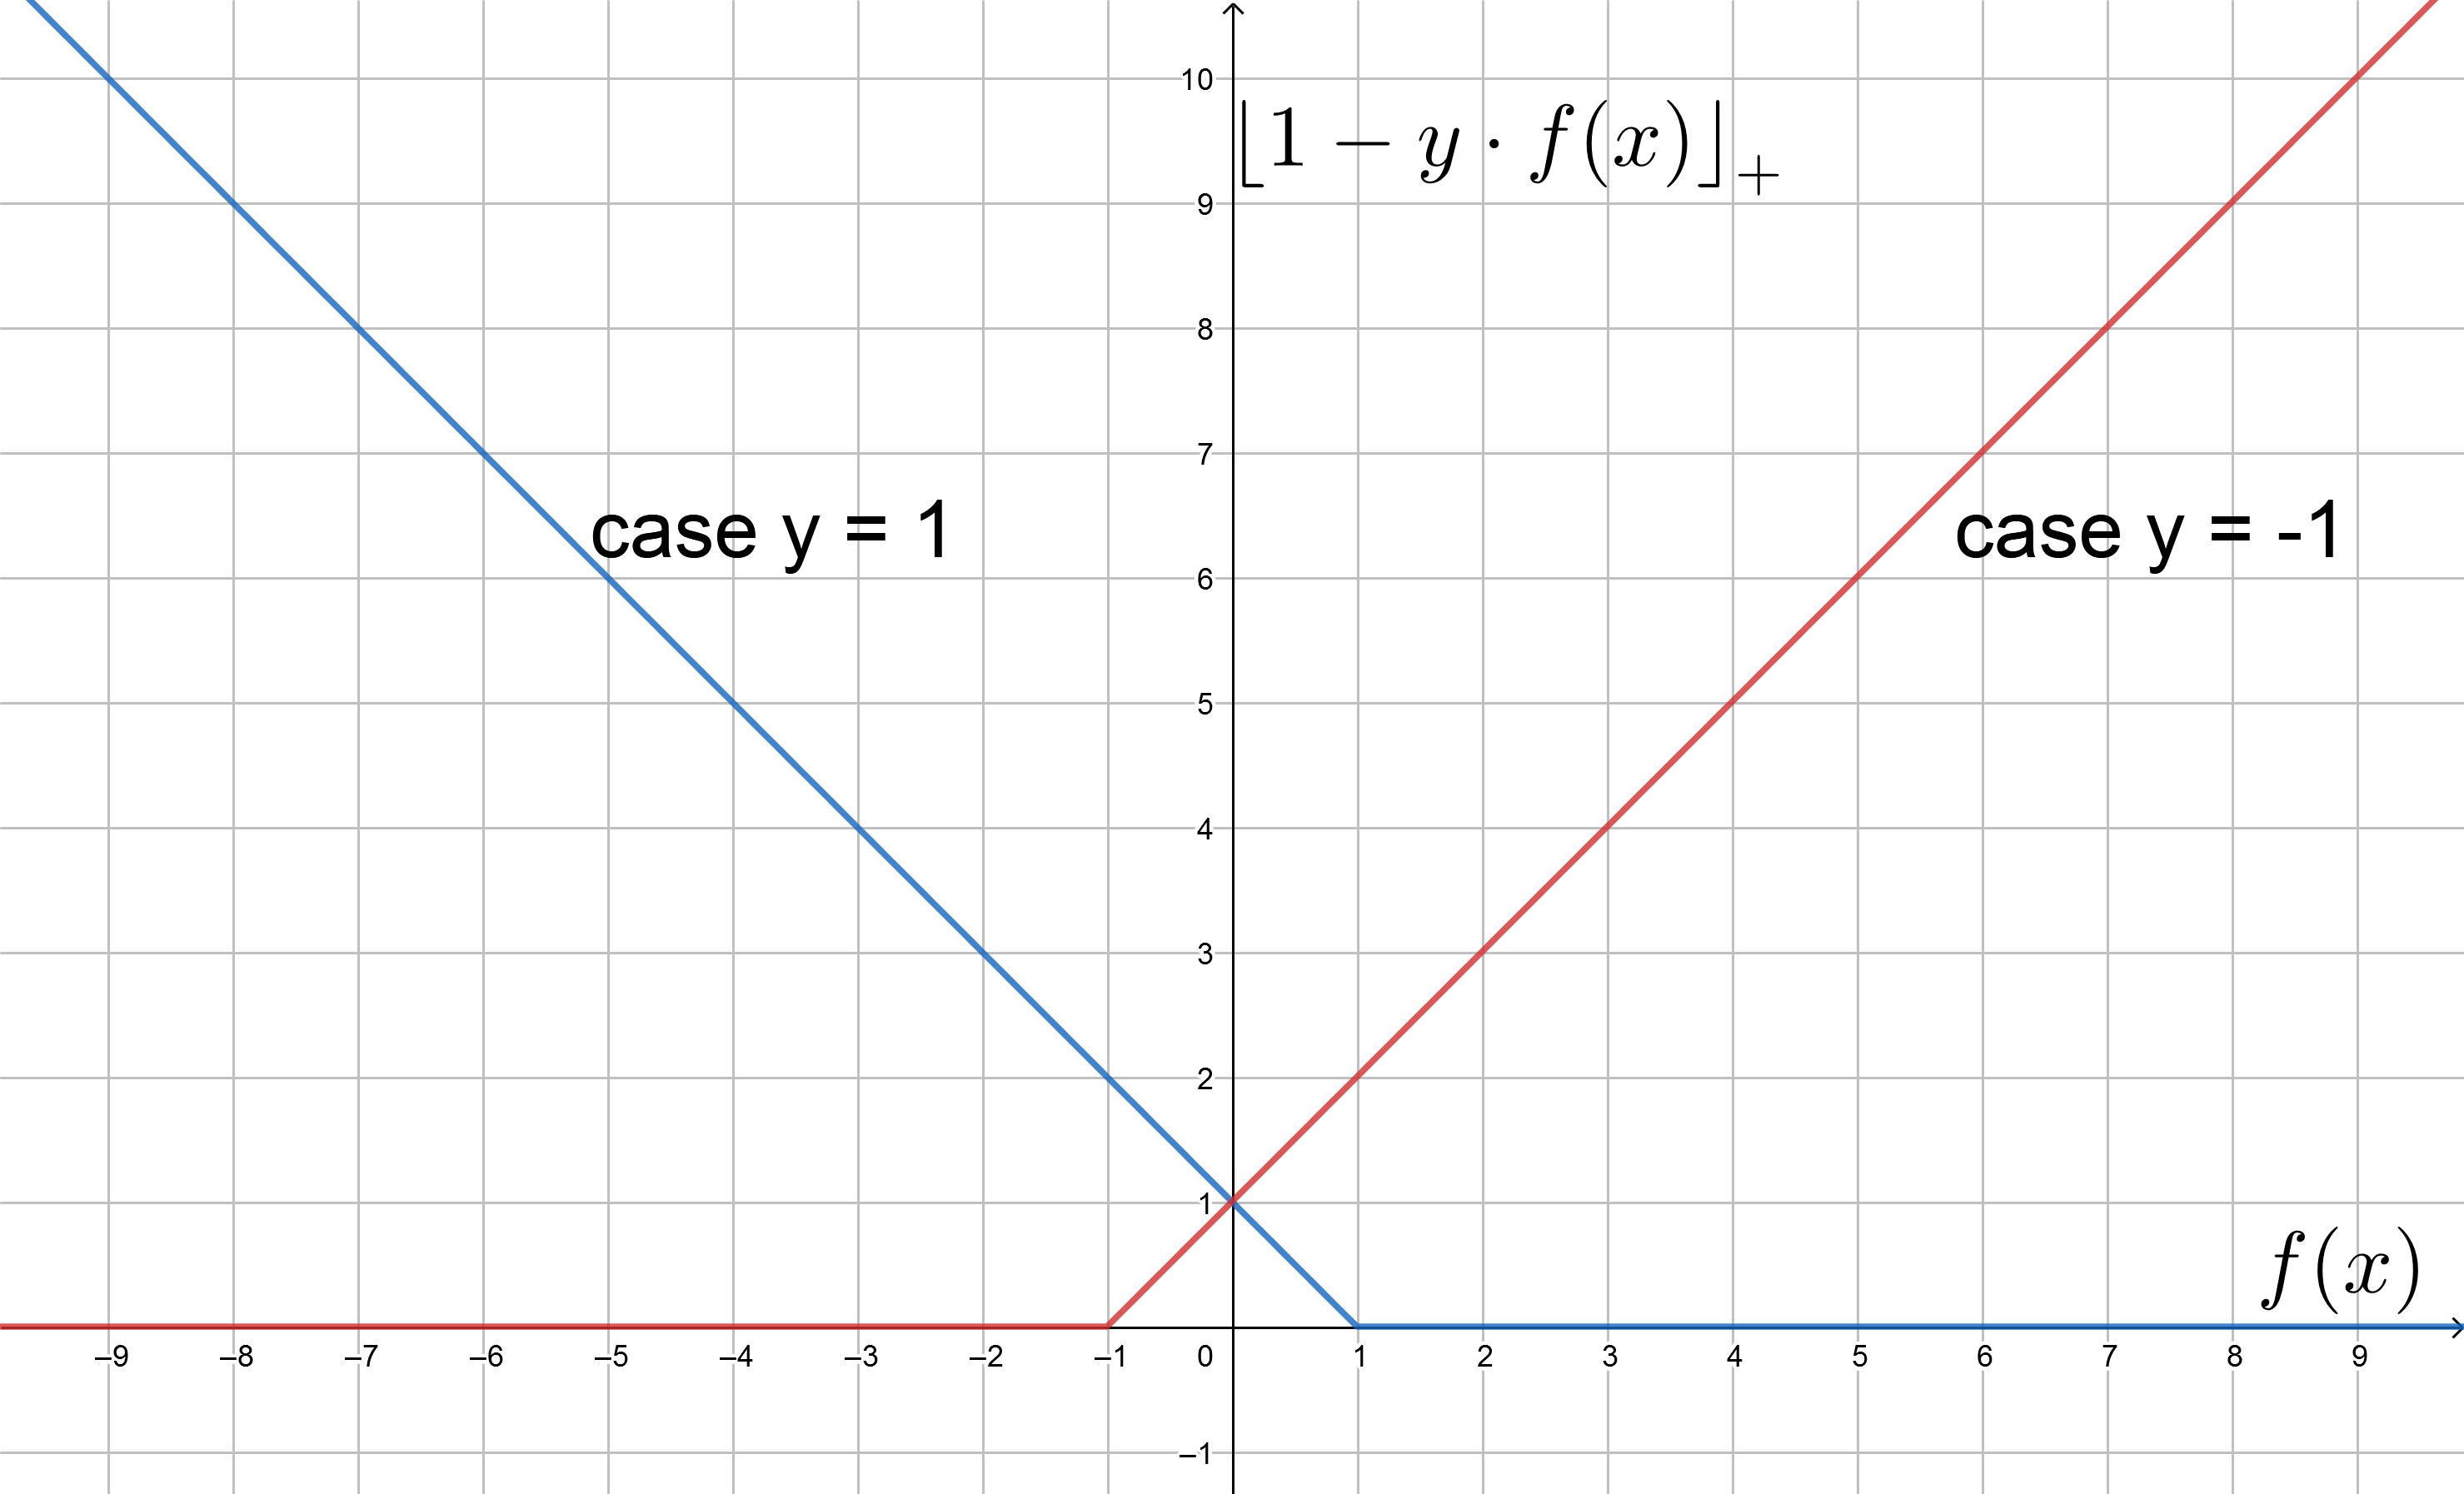
\includegraphics[width=0.7\linewidth]{images/svm-error.png}
 	\caption{%
 		الخطأ في العينة الواحدة في نموذج الـ \eng{SVM}.
 	}
 	\label{fig:svm:error}
 \end{figure}

يمكن البرهان على أنه في حالة كون المعطيات قابلة للفصل بخط مستقيم، فإن حل مسألة الأمثلة سيعطي المستقيم $f$ الذي يحقق أكبر هامش ممكن؛
أي اذا قمنا بحساب البعد بين كل نقطة وهذا المستقيم، فإن أصغر بعد سيكون أكبر ما يمكن، وهذا ما يوضحة الشكل~\ref{fig:svm:margin}.
 \begin{figure}[htb]
	\centering
	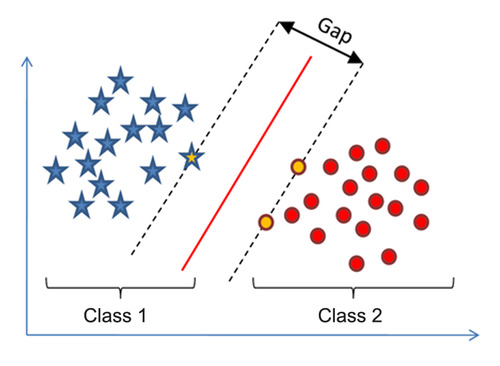
\includegraphics[width=0.5\linewidth]{images/svm-margin.jpg}
	\caption{
		مستقيم يفصل صفين بهامش أعظمي.
	}
	\label{fig:svm:margin}
\end{figure}

ولكن أيضاً يمكننا اختيار تابع غير خطي. هذا مفيد مثلاً في حال كان شكل معطيات التدريب مثلما في الشكل~\ref{fig:svm:non-linear}.
 \begin{figure}[htb]
	\centering
	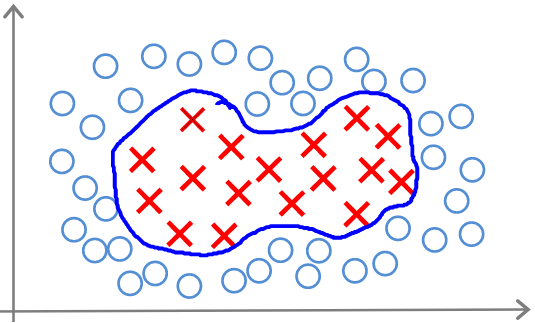
\includegraphics[width=0.5\linewidth]{images/svm-non-linear.PNG}
	\caption{
		معطيات التدريب غير قابلة للفصل باستخدام مستقيم.
	}
	\label{fig:svm:non-linear}
\end{figure}
إذ يوجد أسلوب يسمى بالـ \eng{Kernel Trick}، يسمح لنا بفعل هذا.
ينص هذا الأسلوب على تعريف $f$ بالشكل
$ f(x) = \sum_{i=1}^{m} \theta_i K(x, x^{(i)}) + \theta_0 $%
، ثمّ حل مسألة الأمثلة السابقة ذاتها.
نلاحظ هنا أنه لدينا $ m+1 $ باراميتر عوض الـ $ n+1 $ باراميتر في الحالة السابقة.
و يسمى التابع $K$ بالنواة \eng{Kernel}.
فمثلاً اختيار
 $ K(u, v) = \sum_{j=1}^{n} u_j v_j $
يؤدي إلى حل مكافئ لحل المسألة الموضحة في المعادلة~\ref{eq:svm:primal}. تسمى هذه النواة بالنواة الخطية \eng{Linear Kernel}.
 
إنّ أشهر النوى المستخدمة عادةً هي:
\begin{doublespacing}
	\begin{center}
		\begin{tabular}{r l l}
			النواة الخطية & \eng{Linear Kernel} &
			 $ K(u, v) = u^T v $
			 \\
			 النواة الحدودية & \eng{Polynomial Kernel} &
			 $ K(u, v) = (u^T v + r)^d $
			 \\
			 النواة الغاوسية & \eng{Gaussian Kernel} &
			 $ K(u, v) = \exp{\left( -\gamma \norm{u - v}^2 \right)} $
		\end{tabular}
	\end{center}
\end{doublespacing}
إذ أن الرمز $u^T$ يرمز إلى المنقول وتحديداً فإن
$ u^T =
\left(\begin{smallmatrix}
u_1 \\ \vdots \\ u_n
\end{smallmatrix}\right)^T
= \left( u_1, \dots, u_n \right) $%
. تسمى النواة الغاوسية أيضاً بـ \eng{Radial Basis Function (RBF) Kernel}.
وننوه أن البارمترات المذكورة $ r, d, \gamma $ هي بارامترات فوقية.

لحل مسألة الأمثلة المطروحة، توجد العديد من الخوارزميات. هذا النوع من المسائل، ومسائل الأمثلة بشكل عام هو فرع
مدروس بشكل جيد في الرياضيات تحت اسم \eng{Mathematical Optimization}.
فتوجد العديد من الخوارزميات المستخدمة لحل مسألة الأمثلة المطروحة.
من أشهرها هي خوارزمية
\eng{Sequential Minimal Optimization (SMO)}%
. يتطلب شرحها الخوض في كثير من التفاصيل الرياضية وهو خارج نطاق هذا المشروع.

\subsection{معايير التقييم}
تختلف معايير تقييم صحة نماذج تعلم الآلة باختلاف نوع المسائل التي تقوم بحلها.
سنتحدث في هذه الفقرة عن أهم معايير التقييم المستخدمة في مسائل التصنيف.

بدايةً لنضع بعض الرموز لتبسيط العلاقات الرياضية وتوضيح الأفكار.
كما تحدثنا سابقاً عن معطيات التدريب،
من المعتاد أن توجد معطيات أخرى مستقلة عن معطيات التدريب تسمى بمعطيات الاختبار \eng{Test Set}.
حيث أنه بعد الحصول على النموذج الناتج من خوارزمية تعلم الآلة بتدريبه على معطيات التدريب،
يتم اختبار هذا النموذج على معطيات الاختبار.
سنرمز لها بـ \eng{TS}.
سنرمز لمجموعة عناصرها بـ $ (x_i, y_i) $، حيث $x_i$ هو شعاع الميزات، $y_i$ هو الصف الموافق.
وسنرمز بـ $\hat{y}_i$ للصف الذي تنبأت به خوارزمية تعلم الآلة المستخدمة والتي نرييد تقييمها.
وسنستخدم الرمز $ \abs{\cdot} $ لعدد عناصر مجموعة ما.
فمثلاً إن $ \abs{y_i = c} $ هو عدد العناصر من \eng{TS} التي لها الصف $c$.

الصِحّة \eng{Accuracy} هي المعيار الأشهر. فهي نسبة العينات التي تم تصنيفها بشكل صحيح. أي:
$$ \mathrm{Accuracy} = \frac{ \abs{\hat{y}_i = y_i} }{ \abs{ \mathrm{TS} } } $$

إنّ هذا المعيار غير كافي للتعبير عن مدى قوة النموذج الناتج.
لنتأمل مثال تكون فيه معطيات التدريب فيها صفين فقط.
نسبة ورود الصف الأول هو $1\%$،
مثل حالة تشخيص مرض نادر.
فبإمكاننا بسهولة الحصول على نموذج بدقة $99\%$.
هذا النموذج يتنبأ دائماً بالصف الثاني؛
فلكون ورود عينات تنتمي للصف الأول نادر جداً تكون صحة هذا النموذج عالية.
ولكن من الواضح أن هذا النموذج غير مجدي.
النقاش السابق يدفع لتحديد معايير أخرى للتقيم.

الدقّة \eng{Precision} هي معيار يعبر عن دقّة تصنيف صف معيّن.
دقّة تصنيف الصف $c$ هي نسبة العينات التي صنفت بشكل صحيح في الصف $c$ من بين جميع العينات التي صنفت بالصف $c$.
أي:
$$ \mathrm{Precision\ for\ class\ c} = \frac{ \abs{ \hat{y}_i = c \wedge y_i = c } }
{ \abs{ \hat{y}_i = c } } $$

الإرجاع \eng{Recall} هو معيار يعبر عن مدى استرجاعنا لعينات من صف معيّن.
معيار الإرجاع للصف $c$ هو نسبة العينات التي صنفت بشكل صحيح في الصف $c$ من بين جميع العينات التي هي ضمن الصف $c$ فعلاً.
أي:
$$ \mathrm{Recall\ for\ class\ c} =
\frac{ \abs{ \hat{y}_i = c \wedge y_i = c } }{ \abs{ y_i = c } } $$

المعيار الأخير الذي سنتحدث عنه يسمى بـ \eng{F1-score}.
ينتج من حاجتنا إلى الاعتماد على قيمة عددية واحدة فقط لمقارنة نموذجين معاً.
وهو معيار يجمع بين الدقّة والإرجاع.
النموذج المقترح للجمع بينهما هو:
$$ \mathrm{F1-score} = 2 \cdot \frac{ \mathrm{Precision} \cdot \mathrm{Recall}}
{\mathrm{Precision} + \mathrm{Recall}} $$
سنرمز لهذا المعيار اختصار بـ \eng{F-score}.
حيث أن الرقم $1$ في اسمه يدل على أننا نعطي للدقّة والإرجاع نفس الأهمية.
فهذا المعيار حالة خاصة من معيار أعم يسمح بإعطاء أهمية أكبر للدقّة على الإرجاع وبالعكس، ولكن لن نتحدث عنه.




 